Επαναλαμβάνεται η διαδικασία εύρεσης της τιμής αντίστασης $R$, προκειμένου να μην εμφανίζεται παραμόρφωση στην έξοδο της γεννήτριας, με διαφορετική αντίσταση $R_2 = 1\kohm$.\par
Αρχικά εκτελείται parametric sweep για $1\kohm\leqslant R\leqslant 101\kohm$ με βήμα $10\kohm$. Παρατηρείται η έξοδος του κυκλώματος, $v_{\mathrm{out}}$, στο πεδίο του χρόνου στο διάστημα $\lb 0,2 \rb\unit{\milli\second}$. Τα αποτελέσματα φαίνονται στο διάγραμμα \ref{plot:ask1:q6_1}.

\begin{plot_fig}[H]
	\begin{center}
		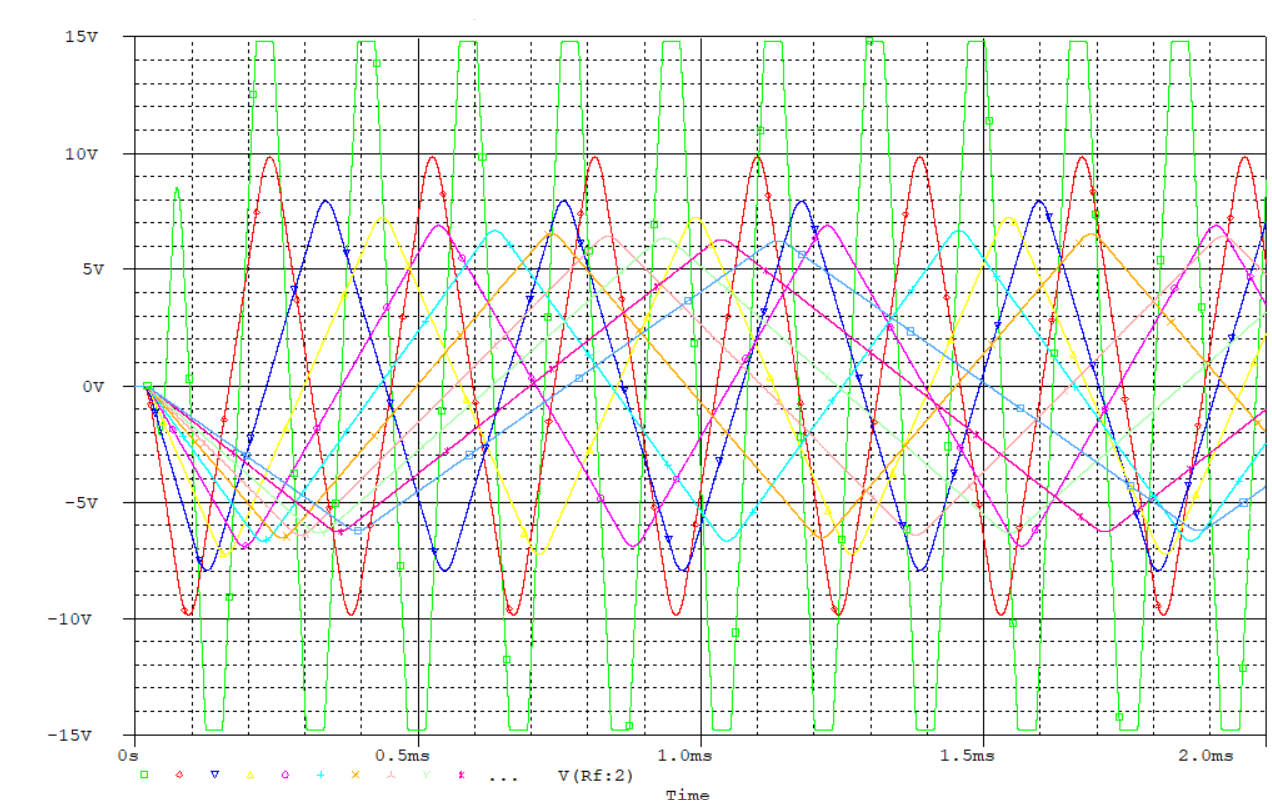
\includegraphics[width=15cm]{spice_01/1.6 a}
		\caption{$v_{\mathrm{out}}$ για $R\in\left\{1,11,\ldots,101\right\}\kohm$.}
		\label{plot:ask1:q6_1}
	\end{center}
\end{plot_fig}

Στο διάγραμμα \ref{plot:ask1:q6_1} παρατηρείται παραμόρφωση της κυματομορφής $v_{\mathrm{out}}$ μόνο για την τιμή $R=1\kohm$. Επόμενο βήμα είναι η παραμετρική ανάλυση για $1\kohm\leqslant R\leqslant 11\kohm$ με βήμα $2\kohm$. Σε αντίθεση με προηγουμένως, συν της $v_{\mathrm{out}}$ παρατηρείται και η $v_2$ προκειμένου να βρεθεί με μεγαλύτερη ακρίβεια η τιμής της $R$ για την οποία υπάρχει παραμόρφωση. Τα αποτελέσματα δίδονται στο διάγραμμα \ref{plot:ask1:q6_2}.

\begin{plot_fig}[H]
	\begin{center}
		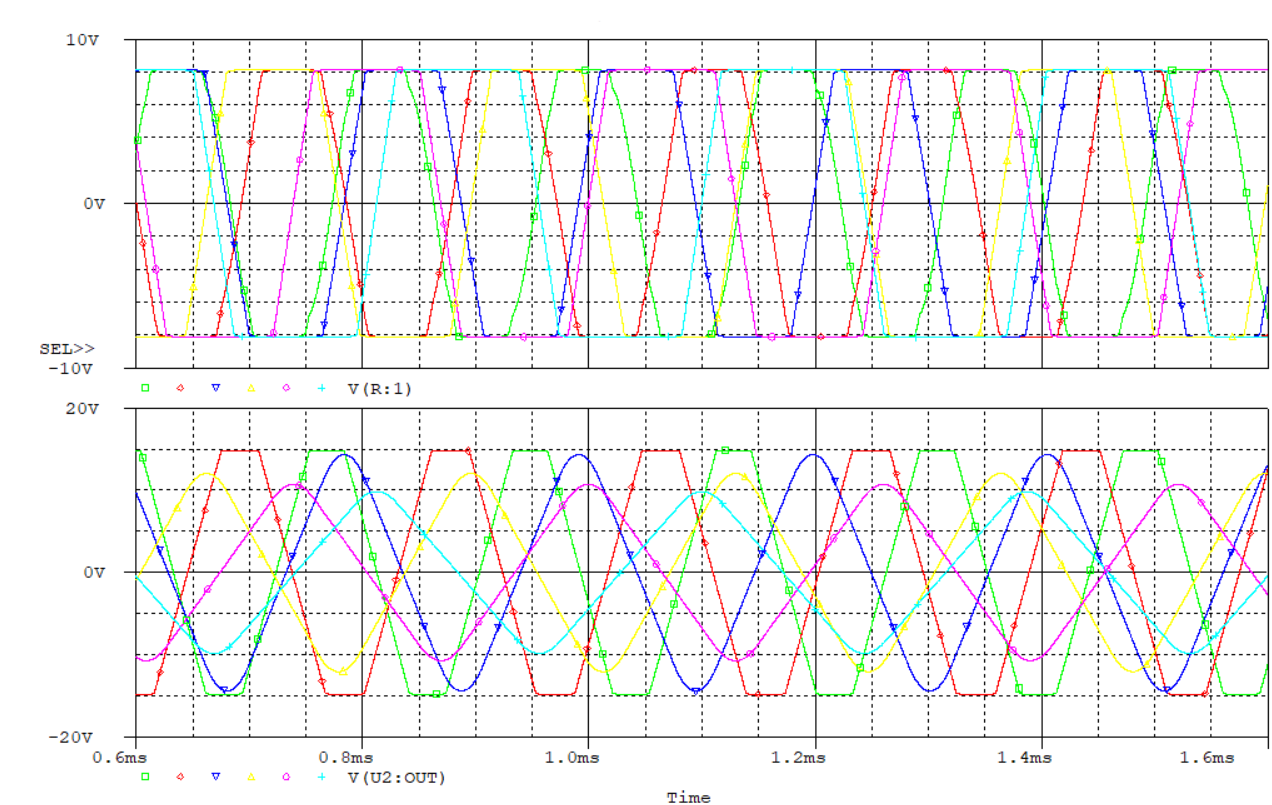
\includegraphics[width=13.5cm]{spice_01/1.6 b}
		\caption{\textsl{Άνω διάγραμμα}: $v_2$ (\texttt{V(R:1)}) για $R\in\left\{1,3\ldots,11\right\}\kohm$. \textsl{Κάτω διάγραμμα}: $v_{\mathrm{out}}$ (\texttt{V(U2:OUT)}) για $R\in\left\{1,3\ldots,11\right\}\kohm$.}
		\label{plot:ask1:q6_2}
	\end{center}
\end{plot_fig}

Έντονη παραμόρφωση παρουσιάζεται στην κόκκινη κυματομορφή για την τάση $v_{\mathrm{out}}$ η οποία αντιστοιχεί σε $R=3\kohm$. Συνεπώς, η προσομοίωση επαναλαμβάνεται για $3\kohm\leqslant R\leqslant 5\kohm$ με βήμα $0.5\kohm$.

\begin{plot_fig}[H]
	\begin{center}
		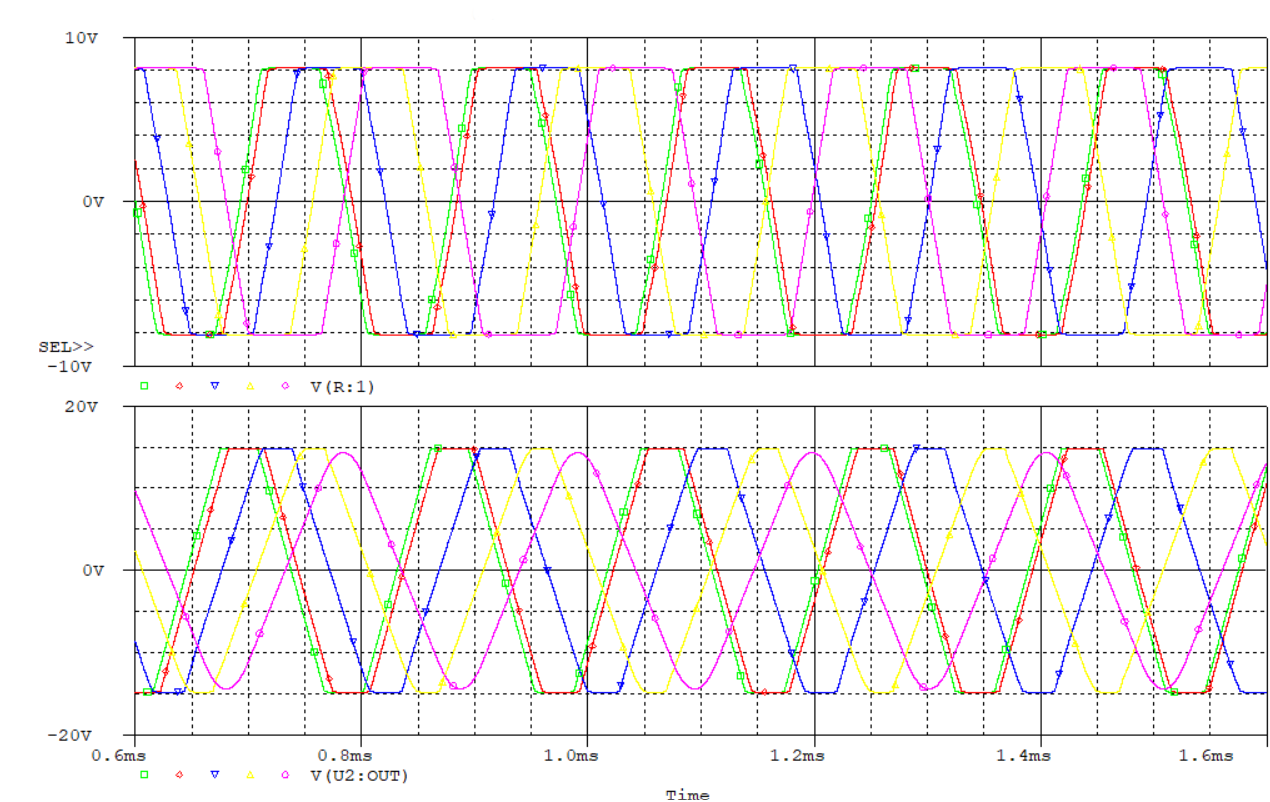
\includegraphics[width=13.5cm]{spice_01/1.6 c}
		\caption{\textsl{Άνω διάγραμμα}: $v_2$ (\texttt{V(R:1)}) για $R\in\left\{3,3.5\ldots,5\right\}\kohm$. \textsl{Κάτω διάγραμμα}: $v_{\mathrm{out}}$ (\texttt{V(U2:OUT)}) για $R\in\left\{3,3.5\ldots,5\right\}\kohm$.}
		\label{plot:ask1:q6_3}
	\end{center}
\end{plot_fig}

% \newpage
Η παραμόρφωση γίνεται αισθητή στην κίτρινη κυματομορφή της $v_{\mathrm{out}}$ η οποία αντιστοιχεί σε $R=4.5\kohm$. Επομένως, η ελάχιστη τιμή της $R$ για την οποία δεν παρουσιάζεται παραμόρφωση θεωρείται η $R=5\kohm$ και οι κυματομορφές των $v_{\mathrm{out}}$ και $v_2$ για αυτή την  τιμή της $R$ φαίνονται στο διάγραμμα \ref{plot:ask1:q6_4}.

\begin{plot_fig}[H]
	\begin{center}
		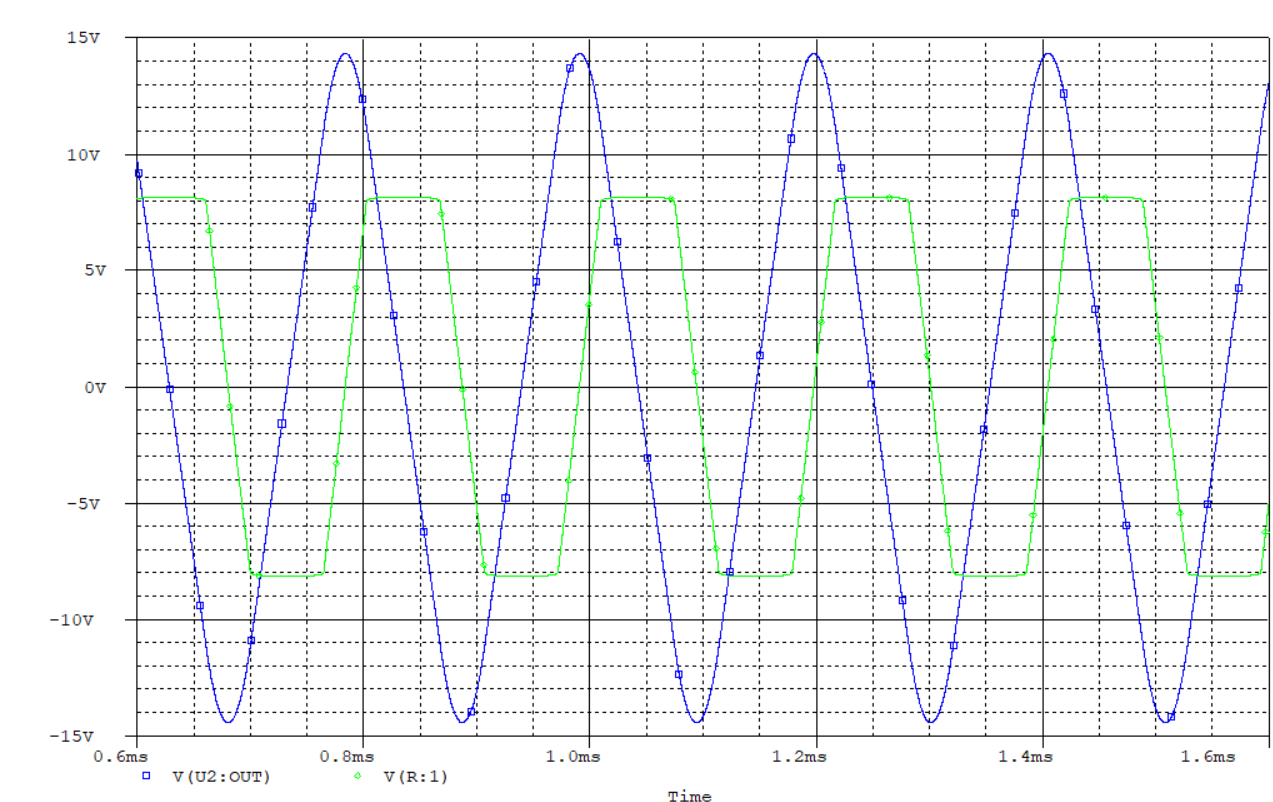
\includegraphics[width=15cm]{spice_01/1.6 d}
		\caption{$v_2$ (\texttt{V(R:1)}) και $v_{\mathrm{out}}$ (\texttt{V(U2:OUT)}) για $R=5\kohm$.}
		\label{plot:ask1:q6_4}
	\end{center}
\end{plot_fig}

Οι περίοδοι των $v_{\mathrm{out}}$ και $v_2$ μετρήθηκαν και βρέθηκαν $T_{\mathrm{out}}=207.043\unit{\micro\second}$. Συνεπώς, η συχνότητα είναι $f_{\mathrm{out}}=4.8299\unit{\kilo\hertz}$. Σε σχέση με την τιμή της $R_2$ στην προηγούμενη ενότητα, παρατηρείται αύξηση της συχνότητας κατά $\sim0.4\unit{\kilo\hertz}$. Μειώνοντας την τιμή της $R_2$ μειώνεται και η πτώση τάσης στα άκρα της. Συνεπώς, η $V_2$ πλησιάζει περισσότερο στην έξοδο του πρώτου τελεστικού ενισχυτή.\par